% Copyright (C) 2018 by latexstudio <http://www.latexstudio.net>
%
% This program is free software: you can redistribute it and/or modify
% it under the terms of the GNU General Public License as published by
% the Free Software Foundation, either version 3 of the License, or
% (at your option) any later version.
%
% This program is distributed in the hope that it will be useful,
% but WITHOUT ANY WARRANTY; without even the implied warranty of
% MERCHANTABILITY or FITNESS FOR A PARTICULAR PURPOSE.  See the
% GNU General Public License for more details.
%
% You should have received a copy of the GNU General Public License
% along with this program.  If not, see <http://www.gnu.org/licenses/>.
%

\section{绘图篇}


\faq{如何利用Tikz画超过360º的角,并做好标注}{}

下面解答来自\url{https://tex.stackexchange.com/questions/60295/drawing-angles-greater-than-360\%C2\%BA-intikz}

\begin{verbatim}
\documentclass[11pt]{scrartcl}
\usepackage{tikz}
\usetikzlibrary{arrows}
\begin{document}
\newcommand\bigangle[2][]{%
\draw[->,domain=0:#2,variable=\t,samples=200,>=latex,#1]
plot ({(\t+#2)*cos(\t)/(#2)},
{(\t+#2)*sin(\t)/(#2)}) node[right=.5cm] {$#2^\circ$}
;}
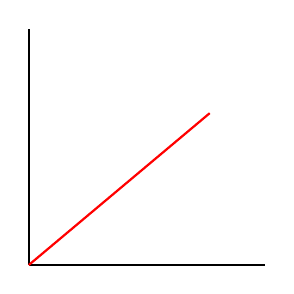
\begin{tikzpicture}
\draw [thick] ( 0,0) -- (3,0);
\draw [thick] ( 0,0) -- (0,3);
\draw [red,thick] ( 0,0) -- (400:3);
\bigangle[blue,dashed]{400}
\end{tikzpicture}
\end{document}
\end{verbatim}

% \includegraphics{https://i.stack.imgur.com/4RO8Y.png}{图片图片}


\faq{如何画交换图?}{}


\faq{如何在插入的图(\cs{includegraphics}\Arg{...})的特定位置插入符号或图}{}

可以使用 overpic 宏包,在 overpic 环境内进行图形绘制,环境内可以使用
latex 自生 picture 环境的绘图语句进行绘制。以下面给出一个例子:

\begin{verbatim}
\documentclass{article}
\usepackage{graphicx}
\usepackage{overpic}
\begin{document}
\begin{overpic}[width=0.8\textwidth
               %,grid,tics=10 % 取消注释可以产生网格线帮助定位,完成后再将其注释。
               ]{1.png}
  \put(35,10){\LaTeX}
  \put(80,0){\includegraphics[width=0.16\textwidth]{1.png}}
\end{overpic}
\end{document}
\end{verbatim}

下面左边是原图,右边是代码处理后的图片:
% \includegraphics{https://images-cdn.shimo.im/VFe2jSxjmoMZpr2B/1.png!thumbnail}
% \includegraphics{https://images-cdn.shimo.im/4qswwF2P4u44JNYB/2.png!thumbnail}

当然还有一种方法可以使用 tikz 宏包,在 tikzpicture
环境引入图片,并在此基础上进行绘图,这样的优点是绘图语句更为丰富,功能更强大。下面举个例子:

\begin{verbatim}
       ![图片](https://images-cdn.shimo.im/LrJDsfrVZIAerfPW/image.png!thumbnail)  ![图片](https://images-cdn.shimo.im/sVlNCmljor0SctYs/image.png!thumbnail)
\end{verbatim}

第一个为原图,第二个是在原图基础上添加一个标号和边.
其中的格线是用来辅助做图的。

\begin{verbatim}
\documentclass{article}
\usepackage{tikz}
\begin{document}
\pgfdeclarelayer{foreground}
\pgfdeclarelayer{background}
\pgfsetlayers{background,main,foreground}
\begin{tikzpicture}
\begin{pgfonlayer}{background}
\path[xshift=-1.24pt,yshift=4pt]      (0,0) node (o) {
  \includegraphics[width=2.8cm]{graph.pdf}};
\end{pgfonlayer}
\begin{pgfonlayer}{foreground}
    \node at (0,0) [label={[label distance=-2mm]40:$u$}]{};
    \draw[step=.5cm,help lines] (-1.4,-1.4) grid (1.4,1.4);
    \coordinate (A) at (0,1.36);
    \coordinate (B) at (0.91,-1.14);
    \fill[color=red] (B) circle (1pt);
    \draw[line width=0.6pt](A)--(B);
\end{pgfonlayer}
\end{tikzpicture}
\end{document}
\end{verbatim}
